% Fig. 2 -- DD-PINN architecture. Drawn at final print size: 190 mm wide
% (Elsevier double-column width), all text >= 7 pt.
\documentclass[border=0.3mm]{standalone}
\usepackage[T1]{fontenc}
\usepackage{amsmath}
\usepackage{txfonts}
\usepackage{booktabs}
\usepackage{tikz}
\usetikzlibrary{arrows.meta,calc,decorations.pathmorphing}

\definecolor{alC}{RGB}{0,114,178}     % aluminum layer / sub-network 1
\definecolor{ssC}{RGB}{213,94,0}      % stainless steel layer / sub-network 2

\newcommand{\fT}{\fontsize{8.5}{10}\selectfont\bfseries}
\newcommand{\fB}{\fontsize{8}{9.6}\selectfont}
\newcommand{\fS}{\fontsize{7.5}{9}\selectfont}
\newcommand{\fX}{\fontsize{7}{8.4}\selectfont}

\tikzset{
  block/.style={draw=black, line width=0.5pt, fill=black!3, rounded corners=0.6mm},
  ibox/.style={rectangle, draw=black, fill=white, line width=0.45pt, rounded corners=0.4mm,
               minimum height=0.6cm, inner sep=1.5pt, font=\fB},
  flow/.style={-{Stealth[length=1.9mm,width=1.5mm]}, line width=0.7pt, draw=black},
  wire/.style={draw=black!62, line width=0.25pt},
  rulel/.style={draw=black!45, line width=0.3pt},
}

% one sub-network row: {y-centre}{index}{colour}{row label}
\newcommand{\subnet}[4]{%
  \begin{scope}[shift={(0,#1)}]
    \foreach \ya in {0.84,0.48,0.12,-0.24,-0.84}{
      \draw[wire] (1.35,0) -- (1.95,\ya);
      \draw[wire] (3.9,\ya) -- (4.35,0);
      \foreach \yb in {0.84,0.48,0.12,-0.24,-0.84}{
        \draw[wire] (1.95,\ya) -- (2.6,\yb);
        \draw[wire] (2.6,\ya) -- (3.25,\yb);
        \draw[wire] (3.25,\ya) -- (3.9,\yb);}}
    \foreach \xa in {1.95,2.6,3.25,3.9}{
      \foreach \ya in {0.84,0.48,0.12,-0.24,-0.84}{
        \node[circle, draw=#3, fill=#3!14!white, line width=0.5pt,
              minimum size=2.4mm, inner sep=0pt] at (\xa,\ya) {};}
      \foreach \d in {-0.45,-0.54,-0.63}{\fill (\xa,\d) circle (0.5pt);}}
    \node[ibox, minimum width=1.0cm] (in#2) at (0.85,0) {$(x,t)$};
    \node[ibox, minimum width=0.8cm] (hat#2) at (4.75,0) {$\hat{T}_{#2}$};
    \node[ibox, minimum width=2.75cm] (sc#2) at (6.975,0)
      {$T_{#2}=T_{\mathrm{ref}}+T_{\mathrm{scale}}\,\hat{T}_{#2}$};
    \draw[flow] (hat#2.east) -- (sc#2.west);
    \node[font=\fS, anchor=west, inner sep=0pt] at (0.35,1.27) {#4};
  \end{scope}}

\begin{document}
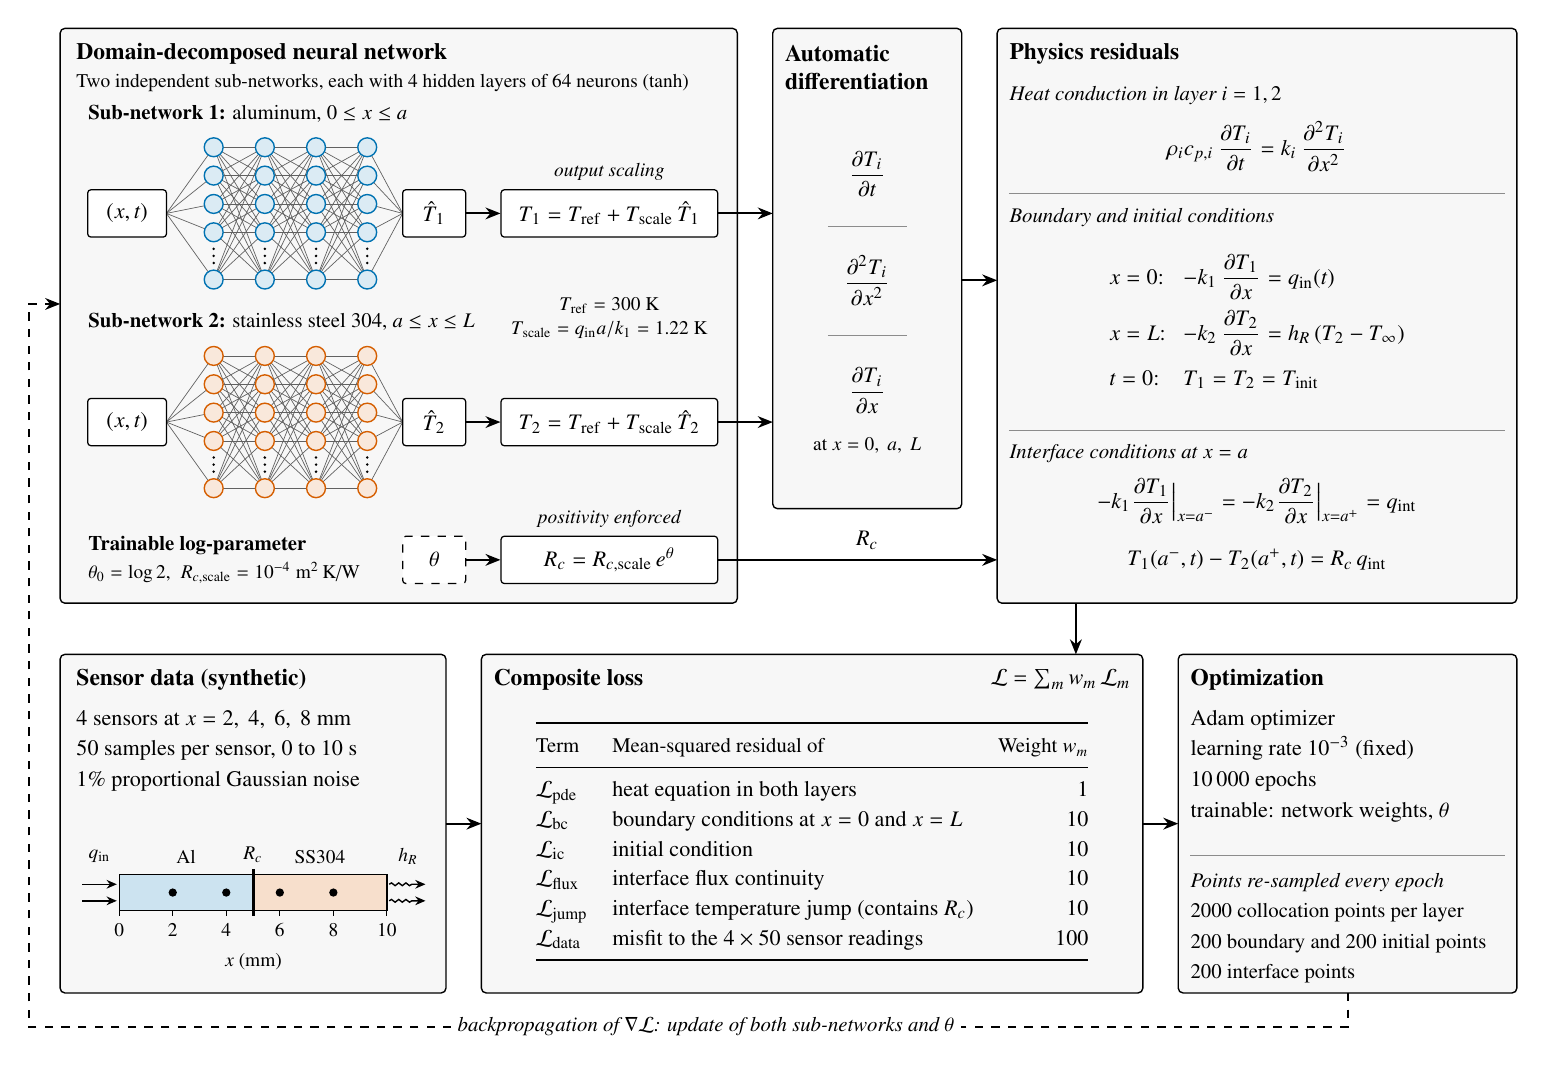
\begin{tikzpicture}[x=1cm,y=1cm]

% ====================== (top left) network ======================
\draw[block] (0,0) rectangle (8.6,-7.3);
\node[font=\fT, anchor=west, inner sep=0pt] at (0.2,-0.32) {Domain-decomposed neural network};
\node[font=\fX, anchor=west, inner sep=0pt] at (0.2,-0.7)
  {Two independent sub-networks, each with 4 hidden layers of 64 neurons (tanh)};

\subnet{-2.35}{1}{alC}{\textbf{Sub-network 1:} aluminum, $0\le x\le a$}
\subnet{-5.0}{2}{ssC}{\textbf{Sub-network 2:} stainless steel 304, $a\le x\le L$}

\node[font=\fX\itshape, inner sep=0pt] at (6.975,-1.82) {output scaling};
\node[font=\fX, align=center, inner sep=0pt] at (6.975,-3.68)
  {$T_{\mathrm{ref}}=300$ K\\[0.5pt]$T_{\mathrm{scale}}=q_{\mathrm{in}}a/k_1=1.22$ K};

% trainable contact-resistance parameter
\node[ibox, minimum width=0.8cm, dashed] (th) at (4.75,-6.75) {$\theta$};
\node[ibox, minimum width=2.75cm] (rc) at (6.975,-6.75)
  {$R_c=R_{c,\mathrm{scale}}\,e^{\theta}$};
\draw[flow] (th.east) -- (rc.west);
\node[font=\fX\itshape, inner sep=0pt] at (6.975,-6.23) {positivity enforced};
\node[font=\fS, anchor=west, align=left, inner sep=0pt] at (0.35,-6.75)
  {\textbf{Trainable log-parameter}\\[1pt]
   {\fX $\theta_0=\log 2$,\; $R_{c,\mathrm{scale}}=10^{-4}$ m$^2$\,K/W}};

% ====================== (top middle) automatic differentiation ======================
\draw[block] (9.05,0) rectangle (11.45,-6.1);
\node[font=\fT, anchor=west, align=left, inner sep=0pt] at (9.2,-0.5)
  {Automatic\\differentiation};
\node[font=\fB] at (10.25,-1.85) {$\dfrac{\partial T_i}{\partial t}$};
\node[font=\fB] at (10.25,-3.2) {$\dfrac{\partial^2 T_i}{\partial x^2}$};
\node[font=\fB] at (10.25,-4.6) {$\dfrac{\partial T_i}{\partial x}$};
\node[font=\fX] at (10.25,-5.3) {at $x=0,\ a,\ L$};
\draw[rulel] (9.75,-2.52) -- (10.75,-2.52);
\draw[rulel] (9.75,-3.9) -- (10.75,-3.9);

\draw[flow] (sc1.east) -- (9.05,-2.35);
\draw[flow] (sc2.east) -- (9.05,-5.0);

% ====================== (top right) physics ======================
\draw[block] (11.9,0) rectangle (18.5,-7.3);
\node[font=\fT, anchor=west, inner sep=0pt] at (12.05,-0.32) {Physics residuals};

\node[font=\fS\itshape, anchor=west, inner sep=0pt] at (12.05,-0.85)
  {Heat conduction in layer $i=1,2$};
\node[font=\fB] at (15.2,-1.5)
  {$\rho_i c_{p,i}\,\dfrac{\partial T_i}{\partial t}=k_i\,\dfrac{\partial^2 T_i}{\partial x^2}$};

\draw[rulel] (12.05,-2.1) -- (18.35,-2.1);
\node[font=\fS\itshape, anchor=west, inner sep=0pt] at (12.05,-2.4)
  {Boundary and initial conditions};
\node[font=\fB] at (15.2,-3.75) {%
  \renewcommand{\arraystretch}{2.1}%
  \begin{tabular}{@{}l@{\hspace{0.8em}}l@{}}
   $x=0$: & $-k_1\,\dfrac{\partial T_1}{\partial x}=q_{\mathrm{in}}(t)$\\
   $x=L$: & $-k_2\,\dfrac{\partial T_2}{\partial x}=h_R\,(T_2-T_\infty)$\\[-4pt]
   $t=0$: & $T_1=T_2=T_{\mathrm{init}}$
  \end{tabular}};

\draw[rulel] (12.05,-5.1) -- (18.35,-5.1);
\node[font=\fS\itshape, anchor=west, inner sep=0pt] at (12.05,-5.4)
  {Interface conditions at $x=a$};
\node[font=\fB] at (15.2,-6.0)
  {$-k_1\dfrac{\partial T_1}{\partial x}\Big|_{x=a^-}=-k_2\dfrac{\partial T_2}{\partial x}\Big|_{x=a^+}=q_{\mathrm{int}}$};
\node[font=\fB] at (15.2,-6.75) {$T_1(a^-,t)-T_2(a^+,t)=R_c\,q_{\mathrm{int}}$};

\draw[flow] (11.45,-3.2) -- (11.9,-3.2);
\draw[flow] (rc.east) -- (11.9,-6.75);
\node[font=\fB, inner sep=1pt] at (10.25,-6.5) {$R_c$};

% ====================== (bottom left) sensor data ======================
\draw[block] (0,-7.95) rectangle (4.9,-12.25);
\node[font=\fT, anchor=west, inner sep=0pt] at (0.2,-8.27) {Sensor data (synthetic)};
\node[font=\fB, anchor=north west, align=left, inner sep=0pt] at (0.2,-8.65)
  {4 sensors at $x=2,\ 4,\ 6,\ 8$ mm\\[1.5pt]
   50 samples per sensor, 0 to 10 s\\[1.5pt]
   1\% proportional Gaussian noise};

% bilayer strip, 0.34 cm per mm
\fill[alC!20!white] (0.75,-10.75) rectangle (2.45,-11.2);
\fill[ssC!20!white] (2.45,-10.75) rectangle (4.15,-11.2);
\draw[line width=0.45pt] (0.75,-10.75) rectangle (4.15,-11.2);
\draw[line width=1.1pt] (2.45,-10.68) -- (2.45,-11.27);
\foreach \m in {2,4,6,8}{\fill ({0.75+0.34*\m},-10.975) circle (1.5pt);}
\foreach \m in {0,2,4,6,8,10}{
  \draw[line width=0.35pt] ({0.75+0.34*\m},-11.2) -- ({0.75+0.34*\m},-11.27);
  \node[font=\fX, inner sep=0pt] at ({0.75+0.34*\m},-11.45) {\m};}
\node[font=\fX, inner sep=0pt] at (2.45,-11.85) {$x$ (mm)};
\node[font=\fX, inner sep=0pt] at (1.6,-10.52) {Al};
\node[font=\fX, inner sep=0pt] at (3.3,-10.52) {SS304};
\node[font=\fX, inner sep=0pt] at (2.45,-10.5) {$R_c$};
\foreach \yy in {-10.87,-11.08}{
  \draw[-{Stealth[length=1.3mm,width=1.1mm]}, line width=0.5pt] (0.28,\yy) -- (0.72,\yy);
  \draw[-{Stealth[length=1.3mm,width=1.1mm]}, line width=0.5pt,
        decorate, decoration={snake,amplitude=0.5pt,segment length=2.6pt,post length=1.3mm}]
        (4.18,\yy) -- (4.64,\yy);}
\node[font=\fX, inner sep=0pt] at (0.5,-10.52) {$q_{\mathrm{in}}$};
\node[font=\fX, inner sep=0pt] at (4.42,-10.52) {$h_R$};

% ====================== (bottom middle) loss ======================
\draw[block] (5.35,-7.95) rectangle (13.75,-12.25);
\node[font=\fT, anchor=west, inner sep=0pt] at (5.5,-8.27) {Composite loss};
\node[font=\fB, anchor=east, inner sep=0pt] at (13.6,-8.27)
  {$\mathcal{L}=\sum_m w_m\,\mathcal{L}_m$};
\node[font=\fB, inner sep=0pt] at (9.55,-10.33) {%
  \renewcommand{\arraystretch}{1.12}%
  \begin{tabular}{@{}l@{\hspace{1.1em}}l@{\hspace{1.1em}}r@{}}
   \toprule
   {\fS Term} & {\fS Mean-squared residual of} & {\fS Weight $w_m$}\\
   \midrule
   $\mathcal{L}_{\mathrm{pde}}$  & heat equation in both layers & 1\\
   $\mathcal{L}_{\mathrm{bc}}$   & boundary conditions at $x=0$ and $x=L$ & 10\\
   $\mathcal{L}_{\mathrm{ic}}$   & initial condition & 10\\
   $\mathcal{L}_{\mathrm{flux}}$ & interface flux continuity & 10\\
   $\mathcal{L}_{\mathrm{jump}}$ & interface temperature jump (contains $R_c$) & 10\\
   $\mathcal{L}_{\mathrm{data}}$ & misfit to the $4\times 50$ sensor readings & 100\\
   \bottomrule
  \end{tabular}};

% ====================== (bottom right) optimization ======================
\draw[block] (14.2,-7.95) rectangle (18.5,-12.25);
\node[font=\fT, anchor=west, inner sep=0pt] at (14.35,-8.27) {Optimization};
\node[font=\fB, anchor=north west, align=left, inner sep=0pt] at (14.35,-8.65)
  {Adam optimizer\\[1.5pt]
   learning rate $10^{-3}$ (fixed)\\[1.5pt]
   10\,000 epochs\\[1.5pt]
   trainable: network weights, $\theta$};
\draw[rulel] (14.35,-10.5) -- (18.35,-10.5);
\node[font=\fS, anchor=north west, align=left, inner sep=0pt] at (14.35,-10.72)
  {\textit{Points re-sampled every epoch}\\[2pt]
   2000 collocation points per layer\\[2pt]
   200 boundary and 200 initial points\\[2pt]
   200 interface points};

% ====================== connections ======================
\draw[flow] (12.9,-7.3) -- (12.9,-7.95);
\draw[flow] (4.9,-10.1) -- (5.35,-10.1);
\draw[flow] (13.75,-10.1) -- (14.2,-10.1);

\draw[flow, dashed] (16.35,-12.25) -- (16.35,-12.68) -- (-0.4,-12.68) -- (-0.4,-3.5) -- (0,-3.5);
\node[font=\fS\itshape, fill=white, inner sep=2.5pt] at (8.2,-12.68)
  {backpropagation of $\nabla\mathcal{L}$: update of both sub-networks and $\theta$};

\end{tikzpicture}
\end{document}
